\documentclass[amsmath, amssymb, aip, jmp, reprint]{revtex4-2}
\usepackage{tikz}
\usetikzlibrary{shapes.geometric}
\usetikzlibrary{decorations.markings}

\begin{document}

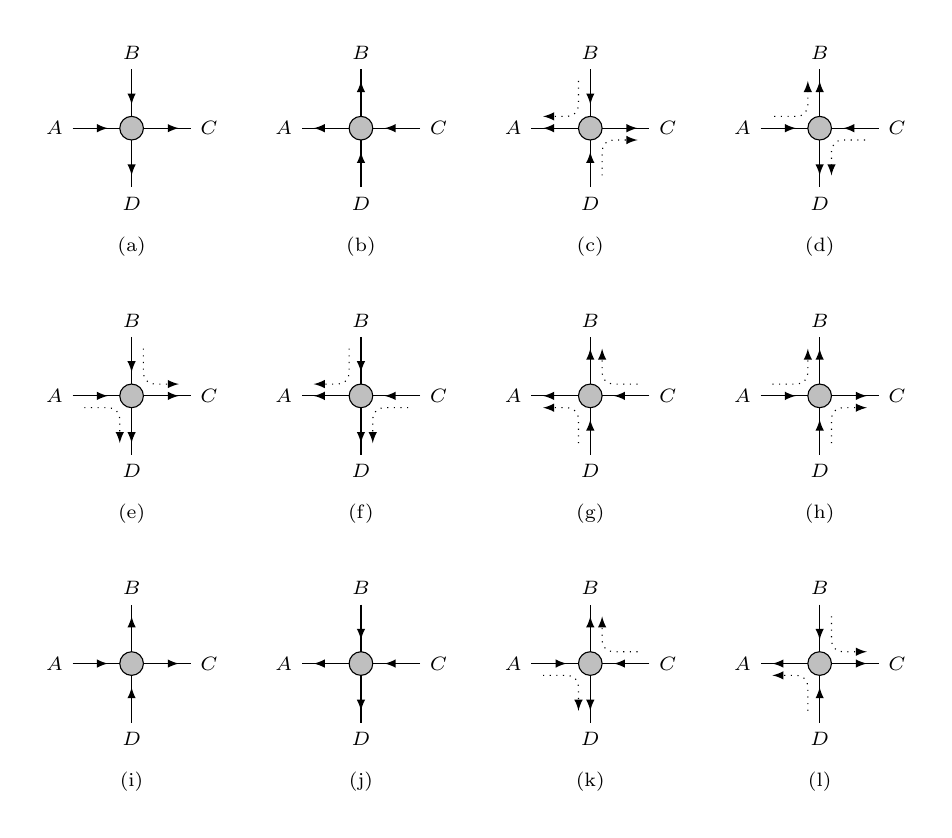
\begin{tikzpicture}[> = latex, font = \scriptsize]
\matrix[column sep = 0.5 cm, row sep = 0.5 cm]{

% Vertex

\draw [fill = gray!50] (0, 0) circle (0.15);

% Connecting edges

\begin{scope}[decoration = {markings, mark = at position 0.75 with {\arrow{latex}}}]

	\draw [postaction = {decorate}] (0.15, 0) -- (0.75, 0) node [right] {$C$};
	\draw [postaction = {decorate}] (-0.75, 0) node [left] {$A$} -- (-0.15, 0);
	\draw [postaction = {decorate}] (0, -0.15) -- (0, -0.75) node [below] {$D$};
	\draw [postaction = {decorate}] (0, 0.75) node [above] {$B$} -- (0, 0.15);

\end{scope}

% Vertex diagram label

\node at (0, -1.5) {(a)};

&

% Vertex

\draw [fill = gray!50] (0, 0) circle (0.15);

% Connecting edges

\begin{scope}[decoration = {markings, mark = at position 0.75 with {\arrow{latex}}}]

	\draw [postaction = {decorate}] (0.75, 0) node [right] {$C$} -- (0.15, 0);
	\draw [postaction = {decorate}] (-0.15, 0) -- (-0.75, 0) node [left] {$A$};
	\draw [postaction = {decorate}] (0, -0.75) node [below] {$D$} -- (0, -0.15);
	\draw [postaction = {decorate}] (0, 0.15) -- (0, 0.75) node [above] {$B$};

\end{scope}

% Vertex diagram label

\node at (0, -1.5) {(b)};

&

% Vertex

\draw [fill = gray!50] (0, 0) circle (0.15);

% Connecting edges

\begin{scope}[decoration = {markings, mark = at position 0.75 with {\arrow{latex}}}]

	\draw [postaction = {decorate}] (0.15, 0) -- (0.75, 0) node [right] {$C$};
	\draw [postaction = {decorate}] (-0.15, 0) -- (-0.75, 0) node [left] {$A$};
	\draw [postaction = {decorate}] (0, -0.75) node [below] {$D$} -- (0, -0.15);
	\draw [postaction = {decorate}] (0, 0.75) node [above] {$B$} -- (0, 0.15);

\end{scope}

% Internal connections

\begin{scope}[->, dotted, rounded corners]

	\draw (-0.15, 0.6) -- (-0.15, 0.15) -- (-0.6, 0.15);
	\draw (0.15, -0.6) -- (0.15, -0.15) -- (0.6, -0.15);

\end{scope}

% Vertex diagram label

\node at (0, -1.5) {(c)};

&

% Vertex

\draw [fill = gray!50] (0, 0) circle (0.15);

% Connecting edges

\begin{scope}[decoration = {markings, mark = at position 0.75 with {\arrow{latex}}}]

	\draw [postaction = {decorate}] (0.75, 0) node [right] {$C$} -- (0.15, 0);
	\draw [postaction = {decorate}] (-0.75, 0) node [left] {$A$} -- (-0.15, 0);
	\draw [postaction = {decorate}] (0, -0.15) -- (0, -0.75) node [below] {$D$};
	\draw [postaction = {decorate}] (0, 0.15) -- (0, 0.75) node [above] {$B$};

\end{scope}

% Internal connections

\begin{scope}[<-, dotted, rounded corners]

	\draw (-0.15, 0.6) -- (-0.15, 0.15) -- (-0.6, 0.15);
	\draw (0.15, -0.6) -- (0.15, -0.15) -- (0.6, -0.15);

\end{scope}

% Vertex diagram label

\node at (0, -1.5) {(d)};

\\

% Vertex

\draw [fill = gray!50] (0, 0) circle (0.15);

% Connecting edges

\begin{scope}[decoration = {markings, mark = at position 0.75 with {\arrow{latex}}}]

	\draw [postaction = {decorate}] (0.15, 0) -- (0.75, 0) node [right] {$C$};
	\draw [postaction = {decorate}] (-0.75, 0) node [left] {$A$} -- (-0.15, 0);
	\draw [postaction = {decorate}] (0, -0.15) -- (0, -0.75) node [below] {$D$};
	\draw [postaction = {decorate}] (0, 0.75) node [above] {$B$} -- (0, 0.15);

\end{scope}

% Internal connections

\begin{scope}[->, dotted, rounded corners]

	\draw (0.15, 0.6) -- (0.15, 0.15) -- (0.6, 0.15);
	\draw (-0.6, -0.15) -- (-0.15, -0.15) -- (-0.15, -0.6);

\end{scope}

% Vertex diagram label

\node at (0, -1.5) {(e)};

&

% Vertex

\draw [fill = gray!50] (0, 0) circle (0.15);

% Connecting edges

\begin{scope}[decoration = {markings, mark = at position 0.75 with {\arrow{latex}}}]

	\draw [postaction = {decorate}] (0.75, 0) node [right] {$C$} -- (0.15, 0);
	\draw [postaction = {decorate}] (-0.15, 0) -- (-0.75, 0) node [left] {$A$};
	\draw [postaction = {decorate}] (0, -0.15) -- (0, -0.75) node [below] {$D$};
	\draw [postaction = {decorate}] (0, 0.75) node [above] {$B$} -- (0, 0.15);

\end{scope}

% Internal connections

\begin{scope}[->, dotted, rounded corners]

	\draw (-0.15, 0.6) -- (-0.15, 0.15) -- (-0.6, 0.15);
	\draw (0.6, -0.15) -- (0.15, -0.15) -- (0.15, -0.6);

\end{scope}

% Vertex diagram label

\node at (0, -1.5) {(f)};

&

% Vertex

\draw [fill = gray!50] (0, 0) circle (0.15);

% Connecting edges

\begin{scope}[decoration = {markings, mark = at position 0.75 with {\arrow{latex}}}]

	\draw [postaction = {decorate}] (0.75, 0) node [right] {$C$} -- (0.15, 0);
	\draw [postaction = {decorate}] (-0.15, 0) -- (-0.75, 0) node [left] {$A$};
	\draw [postaction = {decorate}] (0, -0.75) node [below] {$D$} -- (0, -0.15);
	\draw [postaction = {decorate}] (0, 0.15) -- (0, 0.75) node [above] {$B$};

\end{scope}

% Internal connections

\begin{scope}[->, dotted, rounded corners]

	\draw (-0.15, -0.6) -- (-0.15, -0.15) -- (-0.6, -0.15);
	\draw (0.6, 0.15) -- (0.15, 0.15) -- (0.15, 0.6);

\end{scope}

% Vertex diagram label

\node at (0, -1.5) {(g)};

&

% Vertex

\draw [fill = gray!50] (0, 0) circle (0.15);

% Connecting edges

\begin{scope}[decoration = {markings, mark = at position 0.75 with {\arrow{latex}}}]

	\draw [postaction = {decorate}] (0.15, 0) -- (0.75, 0) node [right] {$C$};
	\draw [postaction = {decorate}] (-0.75, 0) node [left] {$A$} -- (-0.15, 0);
	\draw [postaction = {decorate}] (0, -0.75) node [below] {$D$} -- (0, -0.15);
	\draw [postaction = {decorate}] (0, 0.15) -- (0, 0.75) node [above] {$B$};

\end{scope}

% Internal connections

\begin{scope}[->, dotted, rounded corners]

	\draw (0.15, -0.6) -- (0.15, -0.15) -- (0.6, -0.15);
	\draw (-0.6, 0.15) -- (-0.15, 0.15) -- (-0.15, 0.6);

\end{scope}

% Vertex diagram label

\node at (0, -1.5) {(h)};

\\	

% Vertex

\draw [fill = gray!50] (0, 0) circle (0.15);

% Connecting edges

\begin{scope}[decoration = {markings, mark = at position 0.75 with {\arrow{latex}}}]

	\draw [postaction = {decorate}] (0.15, 0) -- (0.75, 0) node [right] {$C$};
	\draw [postaction = {decorate}] (-0.75, 0) node [left] {$A$} -- (-0.15, 0);
	\draw [postaction = {decorate}] (0, -0.75) node [below] {$D$} -- (0, -0.15);
	\draw [postaction = {decorate}] (0, 0.15) -- (0, 0.75) node [above] {$B$};

\end{scope}

% Vertex diagram label

\node at (0, -1.5) {(i)};

&

% Vertex

\draw [fill = gray!50] (0, 0) circle (0.15);

% Connecting edges

\begin{scope}[decoration = {markings, mark = at position 0.75 with {\arrow{latex}}}]

	\draw [postaction = {decorate}] (0.75, 0) node [right] {$C$} -- (0.15, 0);
	\draw [postaction = {decorate}] (-0.15, 0) -- (-0.75, 0) node [left] {$A$};
	\draw [postaction = {decorate}] (0, -0.15) -- (0, -0.75) node [below] {$D$};
	\draw [postaction = {decorate}] (0, 0.75) node [above] {$B$} -- (0, 0.15);

\end{scope}

% Vertex diagram label

\node at (0, -1.5) {(j)};

&

% Vertex

\draw [fill = gray!50] (0, 0) circle (0.15);

% Connecting edges

\begin{scope}[decoration = {markings, mark = at position 0.75 with {\arrow{latex}}}]

	\draw [postaction = {decorate}] (0.75, 0) node [right] {$C$} -- (0.15, 0);
	\draw [postaction = {decorate}] (-0.75, 0) node [left] {$A$} -- (-0.15, 0);
	\draw [postaction = {decorate}] (0, -0.15) -- (0, -0.75) node [below] {$D$};
	\draw [postaction = {decorate}] (0, 0.15) -- (0, 0.75) node [above] {$B$};

\end{scope}

% Internal connections

\begin{scope}[->, dotted, rounded corners]

	\draw (-0.6, -0.15) -- (-0.15, -0.15) -- (-0.15, -0.6);
	\draw (0.6, 0.15) -- (0.15, 0.15) -- (0.15, 0.6);

\end{scope}

% Vertex diagram label

\node at (0, -1.5) {(k)};

&

% Vertex

\draw [fill = gray!50] (0, 0) circle (0.15);

% Connecting edges

\begin{scope}[decoration = {markings, mark = at position 0.75 with {\arrow{latex}}}]

	\draw [postaction = {decorate}] (0.15, 0) -- (0.75, 0) node [right] {$C$};
	\draw [postaction = {decorate}] (-0.15, 0) -- (-0.75, 0) node [left] {$A$};
	\draw [postaction = {decorate}] (0, -0.75) node [below] {$D$} -- (0, -0.15);
	\draw [postaction = {decorate}] (0, 0.75) node [above] {$B$} -- (0, 0.15);

\end{scope}

% Internal connections

\begin{scope}[->, dotted, rounded corners]

	\draw (-0.15, -0.6) -- (-0.15, -0.15) -- (-0.6, -0.15);
	\draw (0.15, 0.6) -- (0.15, 0.15) -- (0.6, 0.15);

\end{scope}

% Vertex diagram label

\node at (0, -1.5) {(l)};

\\
};
\end{tikzpicture}

\end{document}